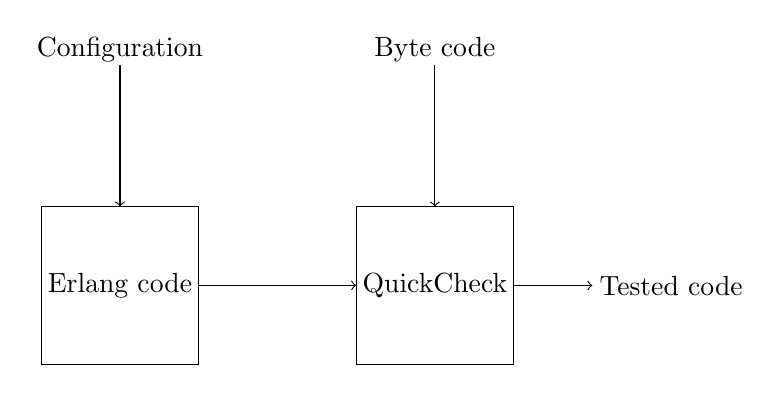
\begin{tikzpicture}
\node at (4,4) {Configuration};
\draw[->] (4,3.8) -- (4,2);
\draw (3,0) rectangle (5,2) node at (4,1) {Erlang code};
\draw[->] (5,1) -- (7,1); %% -> Compiler
\node at (8,4) {Byte code};
\draw[->] (8,3.8) -- (8,2);
\draw (7,0) rectangle (9,2) node at (8,1) {QuickCheck};
\draw[->] (9,1) -- (10,1);
\node at (11,1) {Tested code};
\end{tikzpicture}
